%% assembly_methods.tex
%% Author: Leighton Pritchard
%% Copyright: James Hutton Institute
%% These slides give a short, high-level account of the two dominant 
%% approaches to sequence assembly


% The two main approaches to sequence assembly
\begin{frame}
  \frametitle{Sequence Assembly}
  Two main approaches to read assembly:
  \begin{itemize}
    \item \textbf{Overlap-Layout-Consensus}: Typically used with smaller sets of longer reads (e.g. 454, PacBio, Ion, Nanopore)
    \item \textbf{de Bruijn assembly}: Typically used with many, shorter reads (e.g. Illumina), but also useful for longer reads
  \end{itemize}
  See e.g. Leland Taylor's thesis (\href{http://gcat.davidson.edu/phast/docs/Thesis_PHAST_LelandTaylor.pdf}{http://gcat.davidson.edu/phast/docs/Thesis\_PHAST\_LelandTaylor.pdf}), and PHAST (\href{http://gcat.davidson.edu/phast/index.html}{http://gcat.davidson.edu/phast/index.html}).
\end{frame}

% SUBSECTION: OLC
% A short account of Overlap-Layout-Consensus
\subsection{Overlap-Layout-Consensus}

% Graphical example of OLC
\begin{frame}
  \frametitle{Overlap-Layout-Consensus}
  \begin{center}
    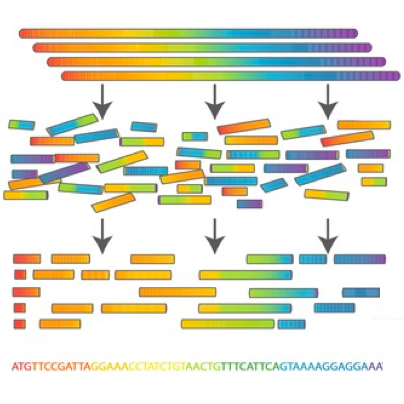
\includegraphics[height=0.8\textheight]{images/overlap-layout-consensus}
  \end{center}  
\end{frame}

% What tools use OLC, for which technologies
\begin{frame}
  \frametitle{Overlap-Layout-Consensus}
  The oldest approach, typically used with smaller sets of fewer reads. \\[0.5cm]
  Can be time consuming (all-vs-all comparisons), but offset with graph-based OLC algorithms (e.g. SGA).\\[0.5cm]
  \begin{itemize}
    \item Celera Assembler\footnote{\tiny{\href{http://wgs-assembler.sourceforge.net/}{http://wgs-assembler.sourceforge.net/}}}
    \item Newbler (the Roche/454 GS assembler)\footnote{\tiny{\href{http://www.454.com/products/analysis-software/}{http://www.454.com/products/analysis-software/}}}
    \item String Graph Assembler\footnote{\tiny{\href{http://dx.doi.org/10.1101/gr.126953.111}{Simpson and Durbin (2012) \textit{Genome Res.} \textbf{22}:549-556 doi:10.1101/gr.126953.111}}}
  \end{itemize}
\end{frame}

% SUBSECTION: de Bruijn graphs
% A short account of de Bruijn graph assembly
\subsection{de Bruijn graph assembly}

% Graphical examples of de Bruijn graphs
\begin{frame}
  \frametitle{de Bruijn graph assembly}
  $k$-mer based graph (choice of $k$ important):
  \begin{center}
    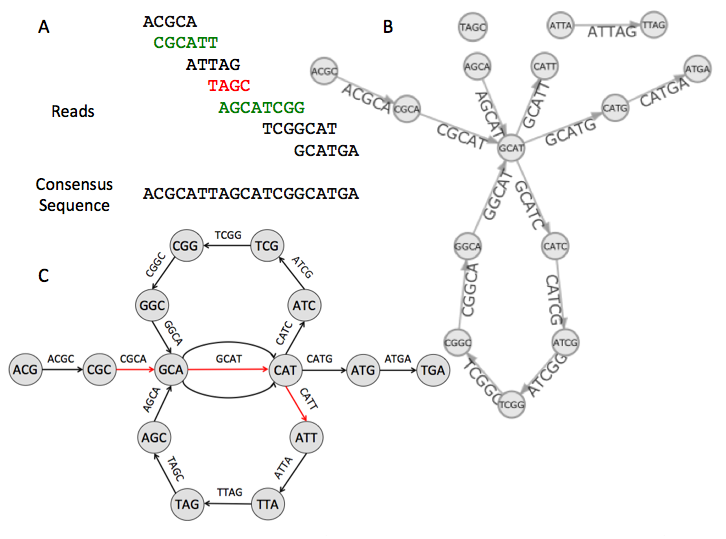
\includegraphics[width=0.8\textwidth]{images/deBruijn3}
  \end{center}  
\end{frame}

\begin{frame}
  \frametitle{de Bruijn graph assembly}
  $k$-mer based graph\footnote{\tiny{\href{http://dx.doi.org/10.1101/gr.079053.108}{Chaisson \textit{et al}. (2009) \textit{Genome Res.} \textbf{19}:336-346 doi:10.1101/gr.079053.108}}}
  \begin{center}
    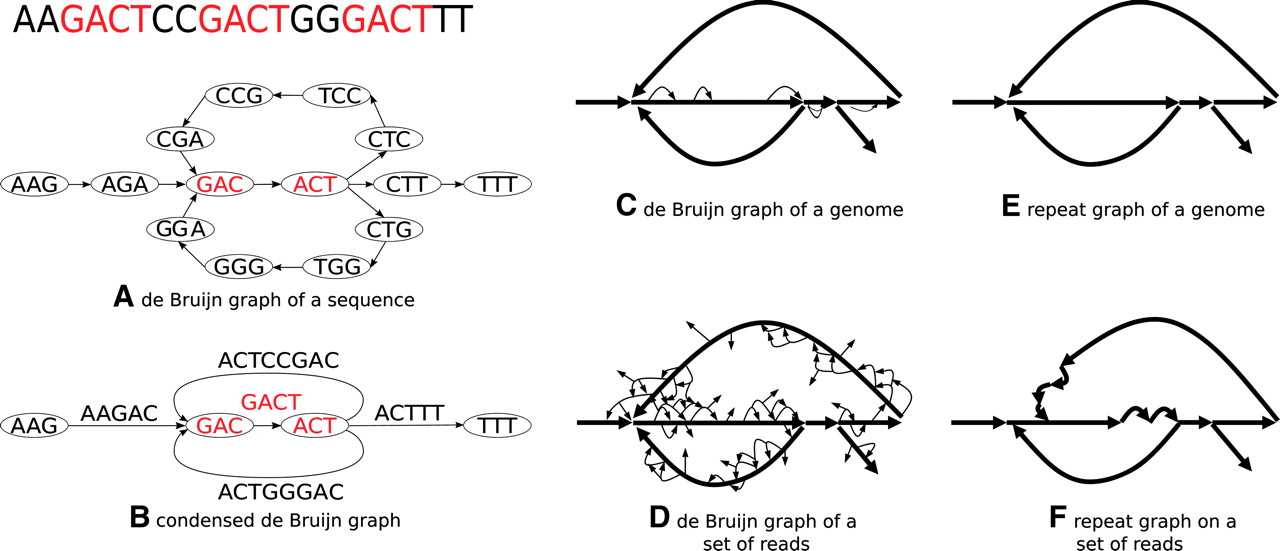
\includegraphics[width=1\textwidth]{images/de_bruijn_repeats}
  \end{center}  
\end{frame}

% What tools use OLC, for which technologies
\begin{frame}
  \frametitle{de Bruijn graph assembly}
  Fast, as it never computes overlaps.\\[0.5cm]
  Sensitive to sequencing errors, and repeats (graph bulges and whirls).\\[0.5cm]
  Notable tools:
  \begin{itemize}
    \item Velvet\footnote{\tiny{\href{http://dx.doi.org/10.1101/gr.074492.107}{Zerbino and Birney (2008) \textit{Genome Res.} \textbf{18}:821-829 doi:10.1101/gr.074492.107}}}
    \item CLC Assembly Cell\footnote{\tiny{\href{http://www.clcbio.com/products/clc-assembly-cell/}{http://www.clcbio.com/products/clc-assembly-cell/}}}
    \item Cortex\footnote{\tiny{\href{http://dx.doi.org/10.1038/ng.1028}{Iqbal \textit{et al}. (2012) \textit{Nat. Genet.} \textbf{44}:226-232 doi:10.1038/ng.1028}}}
  \end{itemize}
\end{frame}

% Graphical example of what else de Bruijn graphs can tell us
\begin{frame}
  \frametitle{``Coloured'' de Bruijn graph assemblies}
  Cortex\footnote{\tiny{\href{http://dx.doi.org/10.1038/ng.1028}{Iqbal \textit{et al}. (2012) \textit{Nat. Genet.} \textbf{44}:226-232 doi:10.1038/ng.1028}}} allows for on-the-fly identification of complex variation, and genotyping, by tracking ``coloured'' edges in the graph.
  \begin{center}
    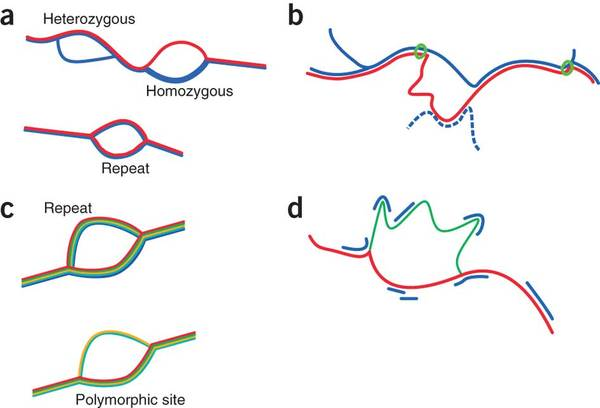
\includegraphics[width=0.8\textwidth]{images/cortex_uses}
  \end{center}  
\end{frame}


